\documentclass{panikzettel}
\usepackage{tikz}
\usepackage{graphicx}
\usepackage{cite}
\usepackage[official]{eurosym}

\title{Entscheidungslehre}
\author{Daniel Sous}

\begin{document}
\maketitle

\tableofcontents

\section{Einleitung}

Dies ist ein kurzer Überblick über die wichtigsten Formeln und Aussagen, die in der Vorlesung \textit{Entscheidungslehre} \cite{vonNitzsch:skript} vorgestellt wurden. Die Zusammenfassung konzentriert sich vor allem auf Formeln und Rechnungen aus den Teilen B \& C. Da es sich um eine Kurzzusammenfassung (aka Panikzettel) handelt, wird auf ausführliche Erklärungen und Herleitungen verzichtet.

Dieser Panikzettel ist Open Source.
Wir freuen uns über Anmerkungen und Verbesserungsvorschläge auf \url{https://git.rwth-aachen.de/philipp.schroer/panikzettel}.

\section{Grundlagen}

\subsection{Bayes-Theorem}
Mit dem Bayes-Theorem lassen sich bedingte Wahrscheinlichkeiten ``umdrehen``:\\
Mit
\begin{align*}
\begin{array}{rrcll}
& P(A | B) & =  & \dfrac{P(A \cap B)}{P(B)} & |\cdot P(B) \\
\Leftrightarrow & P (A|B) \cdot P(B) & = & P(A \cap B)
\end{array}
\end{align*}
und
\begin{align*}
\begin{array}{rrcll}
& P(B | A) & =  & \dfrac{P(A \cap B)}{P(A)} & |\cdot P(A) \\
\Leftrightarrow & P (B|A) \cdot P(A) & = & P(A \cap B)
\end{array}
\end{align*}
folgt
\begin{align*}
	P (A|B) \cdot P(B) = P(A \cap B) = P (B|A) \cdot P(A).
\end{align*}
Durch Umstellen folgt das \textbf{Bayes-Theorem}:
\begin{align*}
	P(A|B) = P(B|A) \cdot \dfrac{P(A)}{P(B)}
\end{align*}

\subsection{Standardnormalverteilung}
Transformation einer Normalverteilung\footnote{Auf weitere Verteilungen wie die Binomialverteilung, Exponentialverteilung, etc. wird hier verzichtet, da diese nicht auswendig zu lernen sind. Der Umgang mit diesen sollte jedoch bekannt sein.} mit Erwartungswert $ \mu $ und Standardabweichung $ \sigma $ (bzw. Varianz $ \sigma^2 $) in eine Standardnormalverteilung $ N(0,1) $ mit $ \mu = 0, \sigma = \sigma^2 = 1 $:
\begin{align*}
	Z &= \frac{X - \mu}{\sigma} \sim N(0,1)\\
	F(x) = P(X \leq x) &= P\left(\frac{X-\mu}{\sigma} \leq \frac{x-\mu}{\sigma}\right) = \phi \left(\frac{x-\mu}{\sigma}\right) = \phi(z)
\end{align*}

\newpage
\section{Präskriptive Entscheidungstheorie}

\subsection{Exponentielle Nutzenfunktion}
\begin{align*}
	u(x) := \begin{cases}
	\dfrac{1 - e ^{-c\frac{x-x^-}{x^+-x^-}}}{1-e^{-c}} & \text{für } c \neq 0\\\\
	\dfrac{x-x^-}{x^+-x^-} & \text{für } c = 0
	\end{cases} && \text{mit } c := -2\text{ln}\left(\frac{1}{p}-1\right)
\end{align*}
Um $ p $ zu ermitteln muss der Entscheider zwischen folgendem sicheren Betrag und dem nebenstehenden Spiel indifferent\footnote{Indifferenz zwischen $A$ und $B$, notiert als $A\sim B$, heißt in diesem Zusammenhang, dass der Entscheider die Entscheidungsmöglichkeiten $A$ und $B$ als gleich gut bewertet.} sein:
\begin{figure}[h]
	\centering
	\begin{tikzpicture}
		\node[](safe) at (-1.2,0) {$ \dfrac{x^-+x^+}{2} $};
		\node[](tilde) at (0,0) {$ \sim $};
		\node[](x+) at (2,0.5) {$ x^+ $};
		\node[](x-) at (2,-0.5) {$ x^- $};

		\path (0.5,0) edge node[auto,scale=0.7,inner sep=0,pos=0.6] {$ p $} (x+);
		\path (0.5,0) edge node[auto,scale=0.7,inner sep=0,swap,pos=0.8] {$ 1-p $} (x-);
	\end{tikzpicture}
\end{figure}\\
Es gilt außerdem
\begin{align*}
c\left\lbrace \begin{array}{cl}
>0 & \text{Risikoscheue}\\
=0 & \text{Risikoneutralität}\\
<0 & \text{Risikofreude}
\end{array}\right.
\end{align*}

\subsection{Erwartungsnutzenmodell}
Eine Alternative $ a $ wird durch $ a := (p_1, a_1; \dots; p_n, a_n) $ definiert, wobei $ p_i $ für die Wahrscheinlichkeit und $ a_i $ für die Ausprägung im Zustand $ i\in\{1, \dots, n\}$ steht. Für den Nutzen der Alternative $ a $ gilt nun
\begin{align*}
	EU(a) := \sum_{i=1}^{n} (p_i \cdot u(a_i))
\end{align*}
mit Nutzenfunktion $ u(x) $. Es wird also der Erwartungswert über die Nutzenwerte gebildet.

\subsection{Additive Nutzenfunktion bei Sicherheit}\label{sec:addUtility}
Bei Sicherheit lässt sich das additive Modell mit $ m $ Zielen und Alternativen $ a = (a_1, \dots, a_m) $ wie folgt definieren
\begin{align*}
	u(a) := \sum_{r=1}^{m} w_r\cdot u_r(a_r) && \text{mit } \sum_{r=1}^{m} w_r = 1 \text{ und } w_r > 0
\end{align*}

\subsection{Additive Nutzenfunktion bei Risiko}
Sei $ a_{ij} $ die Ausprägung der Alternative $ a $ im $ i $-ten Zustand und $ j $-ten Ziel, sowie $ p(s_i) $ die Wahrscheinlichkeit des Umweltzustands $ s_i $, dann gilt:
\begin{align*}
	EU(a) := \sum_{i=1}^{n} p(s_i) \cdot (w_1u_1(a_{i1}) + \dots + w_mu_m(a_{im}))
\end{align*}
Gewichte wie bei \nameref{sec:addUtility}

\subsection{Trade-Off Verfahren}
Sind die Zielgewichte $ w_1, \dots, w_r $ mit $ r\in\mathbb{N} $ gesucht und $ r-1 $ indifferente Präferenzen angegeben, kann das Trade-Off Verfahren angewendet werden, um die Gewichte zu bestimmen. Hier werden die indifferenten Präferenzen gleichgesetzt und nach einem beliebigen Gewicht umgeformt:
\begin{align*}
	w_1u_1(a_1) + \dots + w_ru_r(a_r) = w_1u_1(b_1) + \dots + w_ru_r(b_r)
\end{align*}
Für $ r=2 $ ergibt sich zum Beispiel:
\begin{align*}
	w_1 = \frac{u_2(a_2) - u_2(b_2)}{u_1(b_1) - u_1(a_1)} w_2
\end{align*}
Da $ w_1 + \dots + w_r = 1 $ gilt, lassen sich nun die absoluten Werte der Gewichte berechnen.

\textit{Hinweis:} Falls das entstehende Gleichungssystem überbestimmt ist (d.h. es gibt mehr als $ r-1 $ indifferente Präferenzen), muss überprüft werden, ob eine gültige Lösung für alle Präferenzen besteht. Falls nicht, kann keine additive Nutzenfunktion verwendet werden.

\subsection{Dominanz bei unvollständiger Information}
\begin{itemize}
	\item Bei gegebenen Intervallen $ p^-_i \leq p(s_i) \leq p^+_i $ für alle $ i\in\{1,\dots,n\} $:

	Falls $ \text{min} \left[p(s_1) \cdot (u(a) - u(b)) + \dots + p(s_n) \cdot (u(a) - u(b)) \right] \geq 0$ gilt, dominiert Alternative $ a $ Alternative $ b $. Dabei sind die Wahrscheinlichkeiten $ p(s_1), \dots, p(s_n) $ jeweils aus dem gegebenen Intervall zu wählen, wobei $ p(s_1) + \dots + p(s_n) = 1 $ gelten muss.

	\item Bei gegebener Rangfolge der Wahrscheinlichkeiten:

	Falls nur die Rangfolge der Wahrscheinlichkeiten ($ p(s_1) \geq \dots \geq p(s_n) $) gegeben ist, müssen folgende Punkte gelten, damit eine Dominanz vorliegt:
	\begin{enumerate}
		\item Der Nutzen im wahrscheinlichsten Zustand muss höher sein als der aller anderen Alternativen.
		\item Im Durchschnitt muss der Nutzen der dominierenden Alternative am höchsten sein.
		\item Bei Kumulierung der Nutzenwerte nach absteigender Wahrscheinlichkeit muss die dominierende Alternative im Vergleich zur dominierten Alternative stets besser oder gleich gut sein.
	\end{enumerate}
\end{itemize}

\newpage
\section{Deskriptive Entscheidungstheorie}
\subsection{Verzerrungen in der Informationswahrnehmung \cite{vonNitzsch:211553}}
\begin{itemize}
	\item \textit{Selektive Wahrnehmung:}\\
	Menschen beschränken ihre Wahrnehmung derart, dass Erwartungen eintreffen und eigene Entscheidungen als ``richtig`` erscheinen.
	\item \textit{Kontrast-Effekte:}\\
	Informationen, die mit einer im Kontrast stehenden Information präsentiert werden, werden oft überhöht wahrgenommen.
	\item \textit{Verfügbarkeitsheuristik:}\\
	Informationen, die im Kopf am leichtesten verfügbar sind, bestimmen das Entscheidungs- und Schätzverhalten, d.h. je verfügbarer ein Ereignis ist, desto größer ist seine subjektive Wahrscheinlichkeit. Hat man zum Beispiel vor kurzem von einem Flugzeugunglück erfahren, so würde man die Wahrscheinlichkeit, selbst Opfer eines solchen Unglücks zu werden, überschätzen.
	\item \textit{Mentale Kontenführung:}\\
	Menschen neigen dazu, alle Projekte, an denen sie arbeiten, isoliert in einem zugehörigen ``Mental Account`` zu verbuchen, wobei gegenseitige Abhängigkeiten zwischen diesen vernachlässigt werden. So würde der Verlust einer Konzertkarte im Wert von 100\euro{} anders bewertet als der Verlust von 100\euro{} Bargeld, obwohl der objektive monetäre Verlust derselbe ist.
	\item \textit{Verankerungsheuristik:}\\
	Personen werden bei Schätzungen von Wahrscheinlichkeiten von einem vorgegebenen Anker beeinflusst, wobei gegenseitige Anpassung unter Berücksichtigung weiterer Informationen zu gering ausfällt. (Siehe \nameref{sec:wskgf})
	\item \textit{Repräsentativitätsheuristik:}\\
	Neigung der Menschen, zu schnell in ein Schema-Denken zu verfallen und die Wahrscheinlichkeit von repräsentativen Ereignissen zu überschätzen.
\end{itemize}

\subsection{Wertfunktion}
Die Wertfunktion spiegelt den subjektiven Wert wieder, welcher für einen Gewinn ($ x \geq 0 $) oder einen Verlust ($ x < 0 $) wahrgenommen wird.
\begin{align*}
	v(x) := \begin{cases}
	\sqrt{x} & \text{für } x\geq 0,\\
	-\lambda\sqrt{-x} & \text{für } x < 0
	\end{cases}
\end{align*}
Ein Commitment drückt sich in dem Parameter $ \lambda $ bei Verlusten aus (\textit{Verlustaversion}). Dieser lässt Verluste für $ \lambda > 1 $ noch ``schlimmer`` wirken.

\subsection{Wahrscheinlichkeitsgewichtefunktion} \label{sec:wskgf}
Menschen überschätzen geringe Wahrscheinlichkeiten und überbewerten die absolute Sicherheit. Die allgemeine Wahrscheinlichkeitsgewichtefunktion ist durch $ \pi_{\delta,\gamma}(p) $ gegeben:
\begin{align*}
	\pi_{\delta,\gamma}(p) := \frac{\delta\cdot p^\gamma}{\delta\cdot p^\gamma + (1-p)^\gamma}
\end{align*}
\begin{figure}[h]
	\centering
	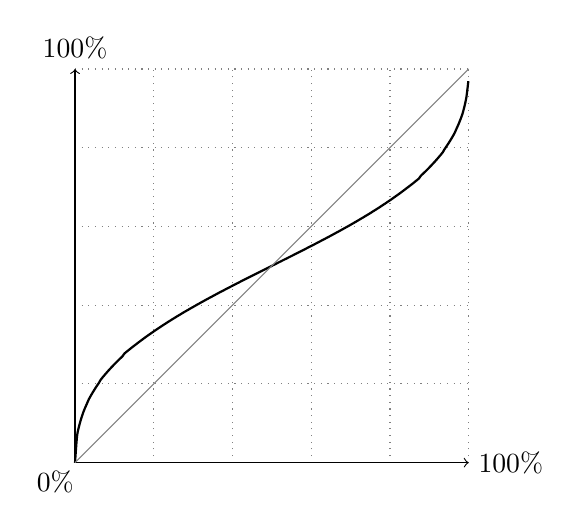
\begin{tikzpicture}[scale=5]
		\draw[dotted,thin,step=0.2,gray] (0,0) grid (1,1);
		\draw[->] (0,0) -- (1,0) node[right] {100\%};
		\draw[->] (0,0) -- (0,1) node[above] {100\%};
		\draw[domain=0:1,smooth,samples=200,variable=\x,thick] plot ({\x},{(\x^0.5)/(\x^0.5 + (1-\x)^0.5)});
		\draw[domain=0:1,variable=\x,gray] plot ({\x}, {\x});
		\node[](zero) at (-0.05,-0.05) {0\%};
	\end{tikzpicture}
	\caption{Graph der Funktion $ \pi_{1,0.5}(p) $}
\end{figure}

\subsection{Risikoeinstellung}
Sei eine sichere Alternative $ A $ und ein Spiel $ B $ - mit Wahrscheinlichkeit $ p_1 $ einen Betrag $ b_1 $ und mit Wahrscheinlichkeit $ p_2 $ einen Betrag $ b_2 $ zu gewinnen - gegeben. Des Weiteren sei eine Wertfunktion $ v(x) $ gegeben. Falls
\begin{align*}
	v(A) = p_1 \cdot v(b_1) + p_2 \cdot v(b_2)
\end{align*}
gilt, dann folgt
\begin{align*}
\begin{array}{ccll}
A & \succ & B\footnotemark & \Rightarrow \text{risikoscheue Einstellung}\\
A & \sim & B & \Rightarrow \text{risikoneutrale Einstellung}\\
A & \prec & B & \Rightarrow \text{risikofreudige Einstellung}\\
\end{array}
\end{align*}
\footnotetext{$ A \succ B $ steht dafür, dass Alternative $ A $ gegenüber Alternative $ B $ bevorzugt wird.}

\subsection{Risikoverhalten}
Um den Begriff des \textit{Risikoverhaltens} zu erläutern, muss zunächst der Begriff \textit{Risikoprämie} definiert werden. Dazu sei ein Spiel mit dem Erwartungswert $ EW $ und ein alternatives Sicherheitsäquivalent $ S\ddot{A} $ gegeben. Dann ist die Risikoprämie $ RP $ definiert als
\begin{align*}
	RP := EW - S\ddot{A}.
\end{align*}
Wird das gegebene Spiel und das Sicherheitsäquivalent als indifferent angesehen, so lässt sich das Risikoverhalten ableiten:
\begin{align*}
	RP \left\lbrace \begin{array}{ccl}
	> & 0 & \text{Entscheider verhält sich risikoscheu}\\
	= & 0 & \text{Entscheider verhält sich risikoneutral}\\
	< & 0 & \text{Entscheider verhält sich risikfreudig}
	\end{array}\right.
\end{align*}
Das Risikoverhalten ist das beobachtbare Verhalten in Risikosituationen. Es bildet das Resultat aus Höhenpräferenzen und Risikoeinstellung.

\subsection{Discounted-Utility-Modell} \label{sec:du}
Der heutige Wert eines zukünftigen Ereignisses wird durch Abdiskontierung seines späteren Nutzens auf den heutigen Zeitpunkt abgebildet:
\begin{align*}
	DU(a) :=& \sum_{t=0}^{T} \left(\frac{1}{1+i}\right)^t u_t(a_t) \\
	=& \sum_{t=0}^{T} e^{-t\cdot \text{ln}(1+i)} u_t(a_t)
\end{align*}
Wobei
\begin{align*}
	u_t(a_t) &= \text{Nutzen des Ergebnisses } a_t \text{ im Zeitpunkt } t\\
	i &= \text{Diskontrate}
\end{align*}
Das Discounted-Utility-Modell ist allerdings ein Modell was sich nur für präskriptive Zwecke eignet, da man hier exponentiell diskontiert (konstante Abnahme der Sensitivität). Dies ist allerdings in der deskriptiven Entscheidungstheorie unrealistisch, weshalb man das \nameref{sec:hdu} verwendet.

\subsection{Hyper\-bolic-Discounted-Utility-Modell} \label{sec:hdu}
Das Hyperbolic-Discounted-Utility-Modell bildet die Sensitivität der Menschen insofern besser ab, dass die Sensitivität zu Beginn stark fällt und dann abflacht.
\begin{align*}
	HDU(a) :=& \sum_{t=0}^{T} \delta^\text{hyp}(t)u_t(a_t)\\
	=& \sum_{t=0}^{T} \left(\frac{1}{1+\alpha t}\right)^{\frac{\beta}{\alpha}} u_t(a_t)
\end{align*}

\begin{figure}[h]
	\centering
	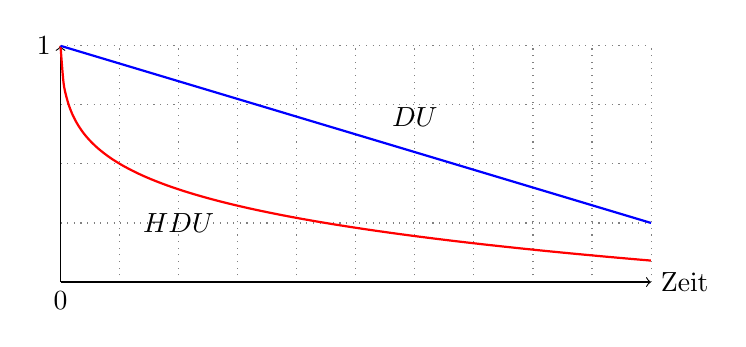
\begin{tikzpicture}[scale=1.5]
		\draw[dotted,thin,step=0.5,gray] (0,0) grid (5,2);
		\draw[->] (0,0) node[left,below] {0} -- (5,0) node[right] {Zeit};
		\draw[->] (0,0) -- (0,2) node [left] {1};
		\draw[domain=0:5,smooth,samples=200,variable=\x,thick,red] plot ({\x},{-(1/1+200*\x)^(30/200) + 3});
		\draw[domain=0:5,smooth,variable=\x,thick,blue] plot ({\x},{-3/10*\x + 2});
		\node[](du) at (3,1.4) {$ DU $};
		\node[](hdu) at (1,0.5) {$ HDU $};
	\end{tikzpicture}
	\caption{Skizze zu \textcolor{blue}{\nameref{sec:du}} und \textcolor{red}{\nameref{sec:hdu}}}
\end{figure}

\newpage
\section{Wege zu einem besseren Entscheiden}
\subsection{Anwendungsfelder der Entscheidungslehre \cite{vonNitzsch:211553}}
\begin{enumerate}
	\item Verbesserung der Entscheidungsqualität
	\item Beeinflussung des Verhaltens Dritter zum eigenen Nutzen
	\item Beeinflussung des Verhaltens Dritter zu deren Nutzen oder zum Nutzen der Gesellschaft (Nudging)
	\item Beeinflussung des eigenen Verhaltens (Selbstlenkung)
	\item Veränderung der Wahrnehmung zur Zufriedenheitssteigerung (Hedonic Framing)
	\item Erlangen eines eigenen Profits aus der Verhaltensprognose anderer
\end{enumerate}

\subsection{Entscheidungen im Team}
Um eine Entscheidung im Team treffen zu können, müssen zunächst die jeweiligen Stakeholder (Personen die ein begründetes Interesse an dem Projekt haben) identifiziert und eingeordnet werden. Dabei muss zwischen den folgenden zwei Aspekten unterschieden werden:
\begin{itemize}
	\item Relative Gewichtung der Ziele des Stakeholders im Verhältnis zu eigenen:

	Hier sollte man sich die Frage stellen, ob derjenige Stakeholder die gleichen Ziele verfolgt und sich damit für das Projekt engagieren wird.

	\item Ausmaß der instrumentellen Bedeutung des Stakeholders für die eigenen Ziele:

	Hier geht es darum, wie viel Einfluss der jeweilige Stakeholder auf die Entscheidung hat. ``Könnte der Stakeholder das Projekt stoppen, wenn er sich nicht einbezogen genug fühlt?\grqq
\end{itemize}
Die Auswertung dieser beiden Aspekte kann nun in einem Netzdiagramm dargestellt werden.

\subsection{Analytisches Vorgehen \cite{vonNitzsch:211553}}
Sowohl für Individual- als auch für Gruppenentscheidungen sollten die folgenden fünf Schritte für ein analytisches Vorgehen berücksichtigt werden:
\begin{enumerate}
	\item[(Z)] Festlegung des Zielkatalogs
	\item[(A)] Alternativensuche
	\item[(EF)] Identifikation der unsicheren Einflussfaktoren
	\item[(P)] Umwelt- und Wirkungsprognosen
	\item[(B)] Analytische Bewertung
\end{enumerate}

\newpage

\subsection{Entscheidungsnavi}
In der Vergangenheit wurden in der Klausur bereits öfters Fragen zum \href{https://entscheidungsnavi.de}{Entscheidungs\-navi} und dessen Struktur gestellt. Unter anderem wurde dort häufig nach den 8 Menüpunkten des Entscheidungs\-navis (Stand: 03.02.2019) gefragt:
\begin{enumerate}
	\item Entscheidungsfrage
	\item Ziele
	\item Alternativen
	\item Unsicherheitsfaktoren
	\item Wirkungsprognosen
	\item Nutzenfunktion
	\item Zielgewichte
	\item Auswertung
\end{enumerate}

% Generated by IEEEtran.bst, version: 1.14 (2015/08/26)
\begin{thebibliography}{1}
	\providecommand{\url}[1]{#1}
	\csname url@samestyle\endcsname
	\providecommand{\newblock}{\relax}
	\providecommand{\bibinfo}[2]{#2}
	\providecommand{\BIBentrySTDinterwordspacing}{\spaceskip=0pt\relax}
	\providecommand{\BIBentryALTinterwordstretchfactor}{4}
	\providecommand{\BIBentryALTinterwordspacing}{\spaceskip=\fontdimen2\font plus
		\BIBentryALTinterwordstretchfactor\fontdimen3\font minus
		\fontdimen4\font\relax}
	\providecommand{\BIBforeignlanguage}[2]{{%
			\expandafter\ifx\csname l@#1\endcsname\relax
			\typeout{** WARNING: IEEEtran.bst: No hyphenation pattern has been}%
			\typeout{** loaded for the language `#1'. Using the pattern for}%
			\typeout{** the default language instead.}%
			\else
			\language=\csname l@#1\endcsname
			\fi
			#2}}
	\providecommand{\BIBdecl}{\relax}
	\BIBdecl

	\bibitem{vonNitzsch:skript}
	\BIBentryALTinterwordspacing
	R.~von Nitzsch, \emph{{Entscheidungslehre : Wie Menschen entscheiden und wie
			sie entscheiden sollten}}.\hskip 1em plus 0.5em minus 0.4em\relax Aachen:
	Mainz, 2017. [Online]. Available: \url{http://d-nb.info/1060414678}
	\BIBentrySTDinterwordspacing

	\bibitem{vonNitzsch:211553}
	\BIBentryALTinterwordspacing
	R.~von Nitzsch, S.~Schiffer, and P.~von Thunen, \emph{Übungen zur
		{E}ntscheidungslehre : Übungsaufgaben und alte {K}lausuraufgaben mit
		{M}usterlösungen, {F}allstudien, {F}achbegriffe; 8. überarbeitete.
		[{A}ufl.]}.\hskip 1em plus 0.5em minus 0.4em\relax Aachen: Mainz, 2017.
	[Online]. Available: \url{http://publications.rwth-aachen.de/record/211553}
	\BIBentrySTDinterwordspacing

\end{thebibliography}

\end{document}
